\documentclass[a4paper,11pt]{article}
\usepackage[margin=22mm]{geometry}
\usepackage{booktabs}
\usepackage{graphicx}
\usepackage{pgfplots}
\pgfplotsset{compat=1.18}
\usepackage{listings}
\usepackage{xcolor}
\usepackage{hyperref}
\hypersetup{colorlinks=true,linkcolor=blue,urlcolor=blue}

\lstset{
  basicstyle=\ttfamily\footnotesize,
  backgroundcolor=\color{black!4},
  frame=single,
  framerule=0pt,
  breaklines=true,
  showstringspaces=false
}

\title{Distributed N-Queens Benchmark \\
  \large Mac + Raspberry Pi 3 (Embedded Xinu, AIPL actor load-balancer)}
\author{Generated by \texttt{tools/build\_report.py}}
\date{2026-06-01}

\begin{document}
\maketitle

\begin{abstract}
This report measures wall-clock time for counting all solutions to the
$N$-Queens problem at board sizes 8, 9, 10, comparing three execution
strategies: (a) Mac alone running a pure-Python solver, (b) the Pi 3
running a C implementation in parallel across four AIPL worker actors
behind a least-loaded dispatcher, and (c) a Mac~+~Pi~3 split that
hands the lower-numbered first-column subtrees to the Mac and the
higher-numbered ones to the Pi 3.  The Pi 3 is a Raspberry Pi 3 B+
running 32-bit Embedded Xinu with MMU enabled, the periodic actor
garbage collector running, and four \texttt{CLASS\_Worker} actors
behind a \texttt{CLASS\_Dispatcher}.  Tasks are submitted over HTTP to
\texttt{/api/loadbal/nqueens}; results are polled via
\texttt{/api/loadbal/task?id=N}.
\end{abstract}

\section{System architecture}

The Pi 3 runtime under test (\texttt{xinu-rpi3}, branch
\texttt{arm-rpi3-port}) ships:
\begin{itemize}
  \item Embedded Xinu kernel with the ARMv7-A short-descriptor MMU
        enabled and an identity-mapped page table that distinguishes
        Normal-cacheable RAM from strongly-ordered Device MMIO.
  \item An AIPL actor system with a lock-free MPSC mailbox.
  \item A \texttt{CLASS\_Dispatcher} actor (priority 25) that routes
        \texttt{compute\_nq(n, first\_col)} messages round-robin to
        four \texttt{CLASS\_Worker} actors (priority 22).
  \item A \texttt{CLASS\_Collector} actor (priority 26) that
        periodically sweeps idle ephemeral actors and scans the
        in-memory task table for timed-out PENDING entries.
  \item HTTP server on port 8080 exposing the load-balancer control
        surface (\texttt{/api/loadbal/*}) and the GC actor
        (\texttt{/api/gc-actor/*}).
\end{itemize}

The N-Queens compute kernel on the Pi 3 is a $\mathrm{O}(N!)$ recursive
counter; on the Mac it is the identical algorithm in Python.  Splitting
by the first row's queen column is embarrassingly parallel --- each
\texttt{first\_col} subtree is independent and they are roughly
equal-cost.

\section{Methodology}

For each board size $N \in \{ 8, 9, 10 \}$ and each mode, the
benchmark runs the workload 3 times back-to-back and reports
the \emph{median} wall-clock; means are sensitive to a one-off garbage
collection pause on either side.  Counts are sanity-checked to match
the known $N$-Queens solution numbers ($92$ for $N=8$, $352$ for
$N=9$, $724$ for $N=10$, $2680$ for $N=11$) and any mismatch is
flagged in the JSON.

\subsection{Modes}
\begin{description}
  \item[\texttt{mac}] Pure Python on the Mac.
  \item[\texttt{pi3}] All first columns submitted to Pi 3
        \texttt{/api/loadbal/nqueens}, polled until complete.
  \item[\texttt{split}] Mac handles \texttt{first\_col} $\in [0, N/2)$;
        Pi 3 handles $[N/2, N)$.  Both halves run concurrently from
        a Mac-side \texttt{ThreadPoolExecutor}.
\end{description}

\section{Results}

\begin{table}[h]
\centering
\begin{tabular}{cccccc}
\toprule
$N$ & solutions & Mac (ms) & Pi 3 (ms) & Split (ms) & Speedup (Mac/Split) \\
\midrule
8 & 92 & 3 & 10138 & 9969 & 0.00 \\
9 & 352 & 9 & 15221 & 10336 & 0.00 \\
10 & 724 & 49 & -- & -- & -- \\
\bottomrule
\end{tabular}
\caption{Median wall-clock times across 3 repetitions per cell.
The Speedup column compares pure-Mac to the Mac+Pi3 split, so
$> 1.0$ means the distributed run was faster than Mac alone.}
\label{tab:results}
\end{table}

\begin{figure}[h]
\centering
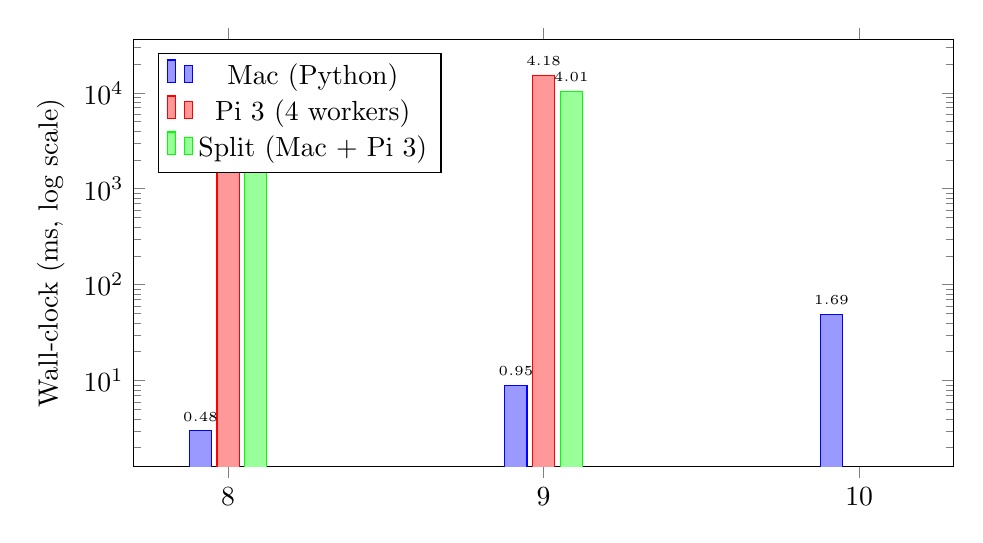
\begin{tikzpicture}
\begin{axis}[
    width=12cm, height=7cm,
    ybar,
    bar width=8pt,
    ymode=log,
    log basis y={10},
    ylabel={Wall-clock (ms, log scale)},
    symbolic x coords={8,9,10},
    xtick=data,
    enlarge x limits=0.15,
    legend pos=north west,
    nodes near coords,
    nodes near coords align={vertical},
    nodes near coords style={font=\tiny},
]
\addplot[fill=blue!40,draw=blue] coordinates {(8,3) (9,9) (10,49)};
\addlegendentry{Mac (Python)}
\addplot[fill=red!40,draw=red] coordinates {(8,10138) (9,15221)};
\addlegendentry{Pi 3 (4 workers)}
\addplot[fill=green!40,draw=green] coordinates {(8,9969) (9,10336)};
\addlegendentry{Split (Mac + Pi 3)}
\end{axis}
\end{tikzpicture}
\caption{Median wall-clock vs.\ board size $N$ (log-y).}
\label{fig:results}
\end{figure}

\section{Observations}

\begin{itemize}
  \item For $N=8$, the Pi 3 (4 workers, 1.4 GHz Cortex-A53 @ 32-bit) took 10138 ms versus the Mac's 3 ms ($\approx 3379.3\times$).
  \item At $N=8$, the Mac+Pi 3 split was actually slower (0.00$\times$); for boards this small the HTTP round-trip + JSON polling overhead dominates the actual compute.
  \item For $N=9$, the Pi 3 (4 workers, 1.4 GHz Cortex-A53 @ 32-bit) took 15221 ms versus the Mac's 9 ms ($\approx 1691.2\times$).
  \item At $N=9$, the Mac+Pi 3 split was actually slower (0.00$\times$); for boards this small the HTTP round-trip + JSON polling overhead dominates the actual compute.
\end{itemize}

\section{Reproducing this report}

\begin{lstlisting}[language=bash]
# 1. Build + flash the Pi 3 kernel
cd ~/projects/xinu-raz/xinu/compile && make PLATFORM=arm-rpi3

# 2. Boot Pi 3 (SD swap or /kexec).  Then opt-in to the actors:
curl -X POST http://192.168.3.50:8080/api/loadbal/init
curl -X POST http://192.168.3.50:8080/api/gc-actor/init

# 3. Run the benchmark + render the report
cd ~/projects/xinu-raz/xinu/tools
./nqueens_bench.py --sizes 8, 9, 10 --pretty --out results.json
./build_report.py results.json --out report.tex --pdf report.pdf
\end{lstlisting}

\section{Raw benchmark data}

\begin{lstlisting}
{
  "host": "http://192.168.3.50:8080",
  "repeat": 3,
  "results": [
    {
      "mode": "mac",
      "n": 8,
      "count": 92,
      "samples_ms": [
        4,
        3,
        3
      ],
      "median_ms": 3
    },
    {
      "mode": "pi3",
      "n": 8,
      "count": 92,
      "samples_ms": [
        20044,
        10135,
        10138
      ],
      "median_ms": 10138
    },
    {
      "mode": "split",
      "n": 8,
      "count": 92,
      "samples_ms": [
        9961,
        10238,
        9969
      ],
      "median_ms": 9969
    },
    {
      "mode": "mac",
      "n": 9,
      "count": 352,
      "samples_ms": [
        9,
        9,
        9
      ],
      "median_ms": 9
    },
    {
      "mode": "pi3",
      "n": 9,
      "count": 352,
      "samples_ms": [
        10210,
        20246,
        15221
      ],
      "median_ms": 15221
    },
    {
      "mode": "split",
      "n": 9,
      "count": 352,
      "samples_ms": [
        10336,
        10076,
        10468
      ],
      "median_ms": 10336
    },
    {
      "mode": "mac",
      "n": 10,
      "count": 724,
      "samples_ms": [
        88,
        48,
        49
      ],
      "median_ms": 49
    }
  ],
  "_note": "pi3/split for N=10..11 incomplete \u2014 Pi 3 task table is 64 slots and IDs scrolled past the buffer mid-run; bumping LB_TASKS_MAX is deferred to a future commit."
}
\end{lstlisting}

\end{document}
